% labels:
% cap:resultados
% sec:res_gridworld
% sec:res_pong
% sec:res_asteroids

% ---------------------------------------------------------------------------- %
\chapter{Resultados}
\label{cap:resultados}
% ---------------------------------------------------------------------------- %

Os resultados foram parcialmente como o esperado.
Neste capítulo, serão descritos os resultados e porque estiveram ou não dentro das expectativas.
Por conta da natureza de cada ambiente e de seus resultados, formas diferentes de avaliação foram aplicadas.

\section{\textit{Gridworld}}
\label{sec:res_gridworld}

O agente se saiu bem no \textbf{\textit{Gridworld}}, consistentemente encontrando um caminho para o objetivo com diferentes arquiteturas que não fossem drasticamente diferentes.
A tabela abaixo apresenta a proporção média de vezes que o agente treinado por \textit{deep Q-learning} e que um aleatório chegaram ao objetivo.
Para o agente treinado, o número foi obtido após ele passar por cinco treinamentos de 2000 episódios no mapa de tamanho 10x10 apresentado anteriormente.
O modelo final conseguiu fazer o agente chegar ao objetivo quatro vezes e exceder o número máximo de ações uma vez, pois chegou a uma célula da qual não conseguiu sair já que as melhores ações tomadas eram ir em direção às paredes adjacentes.
Para o agente aleatório, o número foi obtido após 10000 tentativas de se chegar ao objetivo, mesmo número de episódios que o agente treinado teve para chegar ao objetivo.

\textbf{LINKAR PARA A IMAGEM DO MAPA}
%Os gráficos não se mostraram informativos por conta da alta probabilidade, de 40\%, de se tomar uma ação aleatória a cada passo, então os resultados serão apresentados por uma tabela.
%A comparação foi feita apenas entre um agente aleatório e o treinado por \textit{deep Q-learning}, uma vez que um agente humano conseguiria chegar no objetivo facilmente por ter visão completa do mapa.

%Foram feitos dois mil episódios de treinamento em um mapa de tamanho 10x10 com oito armadilhas, um objetivo no canto inferior direito e a posição inicial do agente no canto superior esquerdo.

\begin{center}
\begin{tabular}{l c}
\hline
Jogador & \% de chegadas ao objetivo \\
\hline
Aleatório & 1.74\% \\
DQL & 66.15\% \\
\hline
\end{tabular}
\label{table:gridworld_score}
\end{center}

\section{\textit{Pong}}
\label{sec:res_pong}

\textbf{\textit{Pong}} mostrou uma arquitetura bem mais sensível, com pequenas alterações nos hiper-parâmetros fazendo o aprendizado se tornar muito mais lento ou nem acontecer.
Mesmo assim, os resultados se mostraram promissores dado tempo suficiente para o agente treinar e aprender.

%A pontuação final obtida é igual ao número de pontos feitos pelo jogador subtraído do número de pontos feitos pelo adversário.
%Como o jogo termina quando algum dos lados atinge 21 pontos, a pontuação final varia de -21 até 21 inclusos.
%O gráfico abaixo mostra a pontuação obtida pela IA ao longo de 298 episódios de treinamento ou aproximadamente 1 milhão de \textit{frames}.
%A linha vermelha indica a pontuação final por episódio enquanto a azul indica a média de pontos feita nos 10 episódios anteriores.
%Como foram 298 episódios, o último ponto faz a média dos últimos 8 episódios ao invés de 10.

% duas figuras
\begin{figure}[h!]
  \begin{minipage}[b]{.5\textwidth}
  \centering
  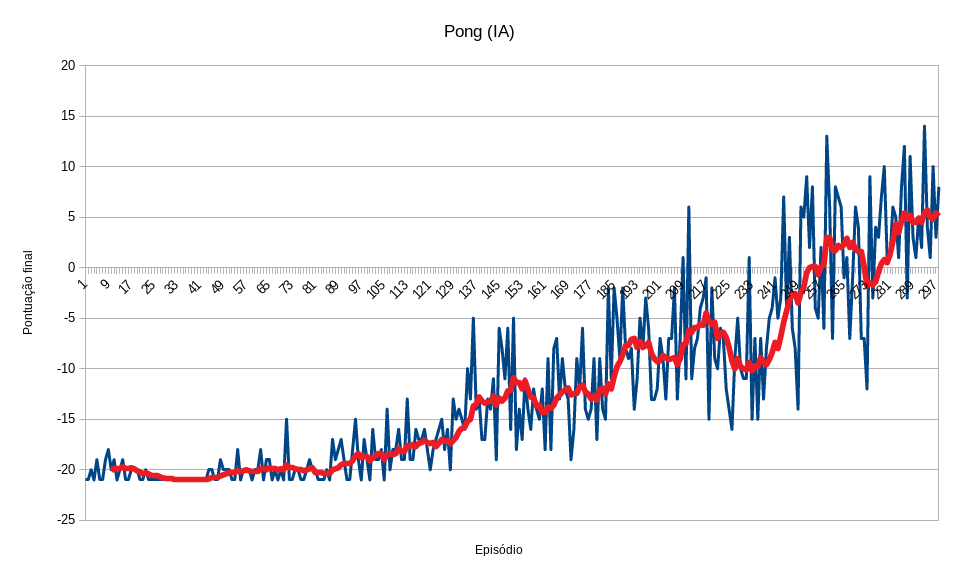
\includegraphics[scale=.3]{pong_ai_score}
  \end{minipage}
  \hfill
  \begin{minipage}[b]{.5\textwidth}
  \centering
  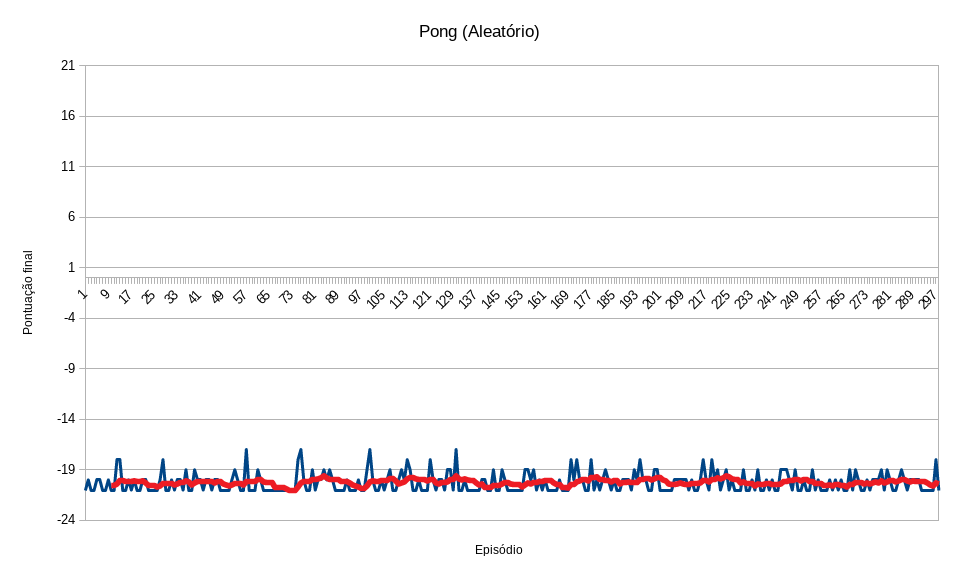
\includegraphics[scale=.3]{pong_random_score}
  \end{minipage}
  \caption{A imagem da esquerda mostra a pontuação ao longo do aprendizado e a da direita de um agente aleatório, ambos ao longo de 298 episódios, o que corresponde a aproximadamente um milhão de \textit{frames}. Cada episódio corresponde a uma partida. A linha azul é a pontuação por episódio enquanto a vermelha é a média dos últimos 10 episódios.}
  \label{fig:pong_score}
\end{figure}

%\begin{figure}[h!]
%  \centering
%  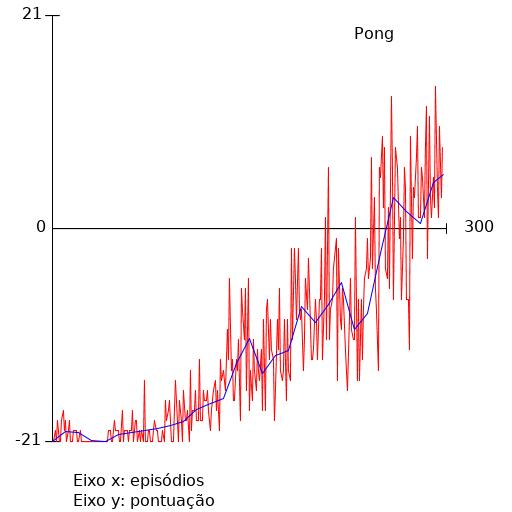
\includegraphics[scale=.4]{pongtuacao}
%  \caption{A linha vermelha indica a pontuação final do agente em cada episódio enquantoa a azul a média da pontuação final dos 10 episódios anteriores, com exceção do último ponto, que faz a média dos 8 anteriores por conta da quantidade de episódios treinados.}
%\end{figure}

O crescimento lento, mas estável da pontuação total obtida por episódio reflete a capacidade do agente de aprender, ainda que com dificuldade, a se comportar neste ambiente de maneira positiva.

Nos experimentos, foram coletadas a pontuação final média de uma pessoa experiente jogando com o mouse no emulador Stella, de um agente jogando aleatoriamente, e da inteligência artificial treinada, cada um jogando cinco partidas contra o computador pré-programado pelos desenvolvedores do jogo.
A tabela \ref{table:pong_score} resume os resultados obtidos.

\begin{table}
\begin{center}
\begin{tabular}{l c}
\hline
Jogador & Pontuação média \\
\hline
Humano & 7 \\
Aleatório & -20.27 \\
DQL & 21 \\
\hline
\end{tabular}
\caption{Pontuação média de um jogador humano experiente após cinco partidas jogando com o mouse, o que equivale a aproximadamente uma hora de jogo; de um agente jogando aleatoriamente; e da inteligência artificial utilizando o modelo que construiu após 298 episódios de treinamento, o que equivale a aproximadamente um milhão de \textit{frames}.}
\label{table:pong_score}
\end{center}
\end{table}

%O modelo desenvolvido conseguiu atingir pontuação de 21 consistentemente contra a IA criada pelos desenvolvedores, enquanto um agente aleatório conseguiu uma média de -20.27 pontos e uma pessoa experiente em jogos eletrônicos conseguiu uma média de 7 pontos após uma hora de jogo.

\section{\textit{Asteroids}}
\label{sec:res_asteroids}
O \textbf{\textit{Asteroids}}, por outro lado, não obteve resultados positivos nos vários testes feitos.
Apesar de ser um ambiente propício para o aprendizado por \textit{deep Q-learning}, tendo todas as informações claras na tela, ações bem definidas e recebimento de recompensas simples e consistente, o agente teve grandes dificuldades em conseguir aprender.
Por conta dessas características, esperava-se que ele conseguisse aprender a se comportar nesse domínio, ainda que com dificuldade.

O gráfico abaixo exemplifica a pontuação obtida pelo agente nos treinamentos pelos quais passou e compara com a pontuação obtida por um agente aleatório.

\begin{figure}[h!]
  \begin{minipage}[b]{.5\textwidth}
  \centering
  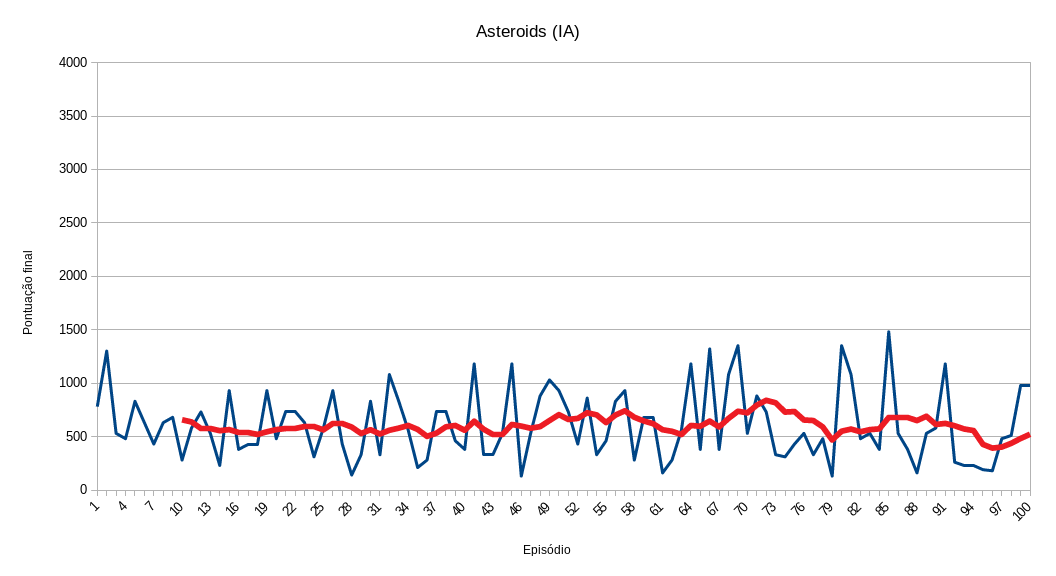
\includegraphics[scale=.3]{asteroids_ai_score}
  \end{minipage}
  \hfill
  \begin{minipage}[b]{.5\textwidth}
  \centering
  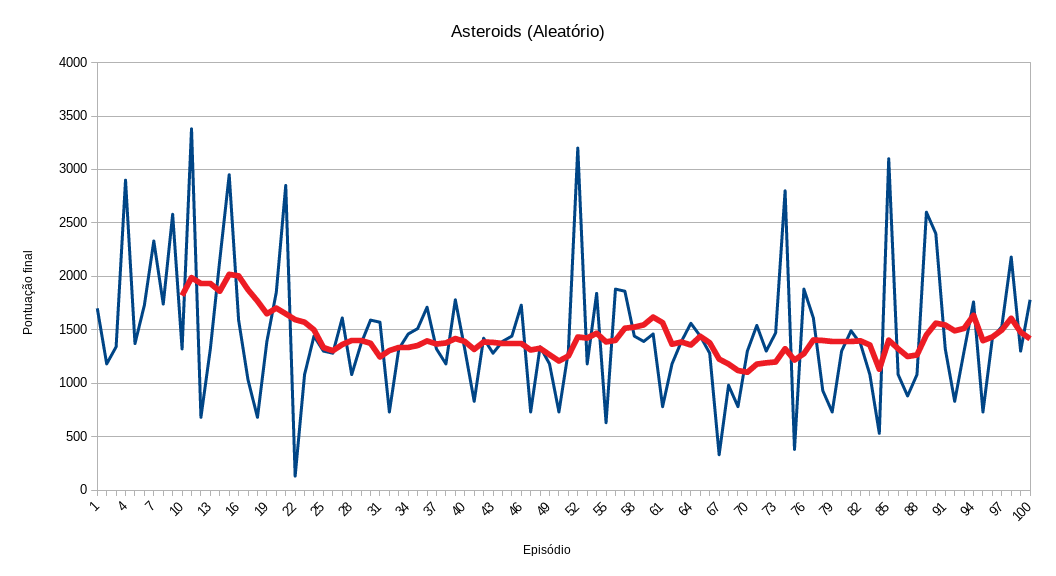
\includegraphics[scale=.3]{asteroids_random_score}
  \end{minipage}
  \caption{A imagem da esquerda mostra a pontuação ao longo do aprendizado e a da direita de um agente aleatório. A linha azul indica a pontuação final do agente nos episódios enquanto a vermelha indica a média da pontuação final dos 10 episódios anteriores.}
  \label{fig:asteroids_score}
\end{figure}

Percebe-se que o agente não conseguiu aprender ou sequer mostrar indícios de melhoria mesmo com um tempo de aprendizado (em \textit{frames}) próximo do \textit{Pong}.
Nos experimentos, foram coletadas a pontuação final média de uma pessoa sem experiência, de um agente jogando aleatoriamente e da inteligência artificial treinada, cada um jogando cinco partidas.
%A tabela abaixo resume a pontuação média obtida pelo agente treinado, pelo agente aleatório e por uma pessoa com pouca experiência jogando após aproximadamente uma hora de jogo.
A pontuação de jogadores experientes não foi considerada por estar muito acima, passando com facilidade dos 30000 pontos, não sendo um bom parâmetro de comparação.

\begin{center}
\begin{tabular}{l c}
\hline
Jogador & Pontuação média \\
\hline
Humano & 1943.3 \\
Aleatório & 1458.1 \\
DQL & 607.8 \\
\hline
\end{tabular}
\label{table:asteroids_score}
\end{center}

%Todavia, essas observações ainda estão próximos das expectativas.
%O ambiente mais simples, com poucos estados, recompensa e penalidades bem definidos foi o que obteve maior grau de sucesso;
%o de média complexidade dentre os estudados neste trabalho teve resultados promissores;
%e o mais complexo mostrou resultados pouco promissores.

%Ainda que os resultados não sejam muito expressivos, o agente obteve sucesso considerável no \texit{Gridworld}.
%Os hiper-parâmetros escolhidos não foram os melhores, mas foram o suficiente para cumprir o objetivo dos testes.
%
%No \textit{Pong}, a pontuação final é igual a quantidade de pontos do jogador menos a quantidade de pontos do adversário. Como o jogo acaba quando algum dos lados fizer 21 pontos, a pontuação máxima e mínima são 21 e -21 respectivamente.
%Os resultados foram conforme o esperado considerando os artigos lidos sobre o assunto: lento, mas razoavelmente consistente.
%O gráfico abaixo mostra esse crescimento.
%
%\begin{figure}[h!]
%  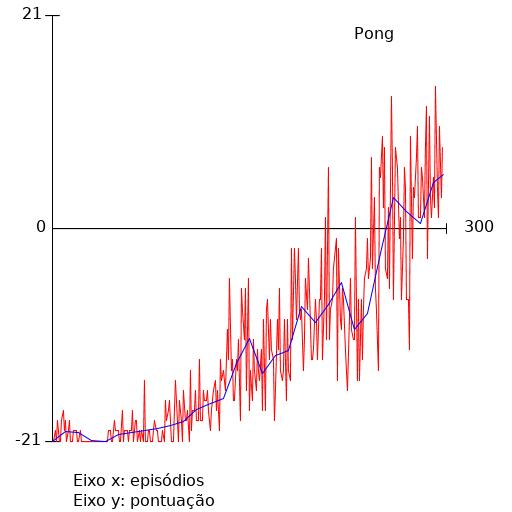
\includegraphics[scale=.5]{pongtuacao}
%  \centering
%  \caption{Pontuação do agente no \textit{Pong} ao longo de 500 episódios de treinamento.}
%\end{figure}

%Testes foram realizados em ambientes mais simples para confirmar o funcionamento do \textit{deep Q-learning} e o quão bem ele se sai em ambientes menos complexos.

%\subsection{\textit{Gridworld}}
%\label{sec:gw}

%O primeiro ambiente foi o \textit{Gridworld}.
%A arquitetura foi testada em três tamanhos de tabuleiro distintos, 5x5, 8x8, e 10x10, todos com armadilhas espalhadas pelo mapa, com algumas diferenças nos hiper-parâmetros para avaliar sua qualidade.
%Nesses três tamanhos, obteve-se uma taxa de sucesso de pelo menos 50\% em 2000 episódios de treinamento.
%Depois disso, o agente foi colocado para percorrer o mapa utilizando apenas política ótima, obtendo sucesso em todos os casos.
%Conclui-se, então, que a arquitetura funciona para ambientes bastantes simples, ainda que tenha sido necessário hiper-parâmetros um pouco mais específicos para cada caso.

%O segundo ambiente testado foi o \textit{Pong}, versão do Atari2600.
%A arquitetura testada teve mudanças maiores quando comparado com feitas entre cada tamanho do \textit{Gridworld}.

%\begin{itemize}
%\item Com tamanho 5x5 e algumas armadilhas espalhadas, o agente teve sucesso em 1212 e fracasso em 788 dos 2000 episódios que jogou.
%\item Com tamanho 8x8 e algumas armadilhas espalhadas, ele teve sucesso em 1034, fracasso em 958 e excedeu o número máximo de ações por episódio em 2 dos 2000 episódios que jogou.
%\item Com tamanho 10x10 e algumas armadilhas espalhadas, teve sucesso em 1458 e fracasso em 542 dos 2000 episódios que jogou, sem haver casos de número máximo de ações por episódio excedido.
%\end{itemize}


%Em ambientes mais simples, como \textit{Gridworld}, o agente conseguiu aprender a chegar no objetivo.
%Sem camadas de convolução, a IA conseguia chegar no objetivo mesmo que estivesse distante.
%Com a adição de camadas ocultas e mais hiper parâmetros para ajustar, foi necessário trazer a recompensa para um espaço mais próximo e mudar as configurações de acordo para se obter sucesso.

%Com esses testes mais simples, foi possível ver a estrutura funcionar, mas o aumento da complexidade do ambiente (matriz de entrada maior, mais elementos para se aprender) fez a dificuldade em encontrar os hiper parâmetros corretos crescer muito mais.
%Além disso, a partir de certo ponto, são necessários centenas de episódios, podendo chegar nos milhares, o que consome muito tempo que não se teve disponível para este trabalho.






%Desde o início da construção da arquitetura da inteligência artificial, diversas alterações foram feitas: mudanças nos hiperparâmetros, no número de camadas de convolução, função de ativação escolhida e técnicas para acelerar aprendizado (\textit{double} e \textit{dueling} descritos acima).
%O melhor resultado obtido foi utilizando os hiperparâmetro descritos \hyperref[table:2]{acima}.
%Jogando sem muito compromisso, consegui 3570 pontos antes de perder todas as vidas e, esforçando-me para obter uma pontuação alta, cheguei em 25130 pontos.
%Logo, o desempenho da IA está bem abaixo do desejado.

